% ======================================================================
% Section 3.2 -- Stakeholder Analysis
% ======================================================================

\section{Stakeholder Identification}
\vspace{-5pt}
\begin{table}[H]
\centering
\vspace{-8pt}
\caption{Stakeholder Identification}
\vspace{-8pt}
\label{tab:stakeholders}
\begin{tabularx}{\textwidth}{@{}cllX@{}}
\toprule
\# & Stakeholder & Type & Interaction \\
\midrule
S1 & Union Parishad (UP) Officials & Primary & Register households, log distributions, view local dashboard \\
S2 & Upazila Officers & Primary & Audit UP-level data, generate reports, manage accounts \\
S3 & NGO Field Workers & Primary & Log distributions, view duplicate alerts \\
S4 & General Public & Primary & View public dashboard (read-only, no login) \\
S5 & District Disaster Management Committee & Secondary & Review aggregated district-level reports \\
S6 & Department of Disaster Management (DDM) & Secondary & Policy-level oversight \\
S7 & Course Teacher (MD Mynoddin) & External & Academic evaluator, QA reviewer \\
S8 & External QA (Saifur Rahman) & External & Independent functionality testing \\
S9 & Team\_Skipper & Internal & Design, build, test, and maintain the system \\
S10 & Affected Households & Indirect & Data subjects; benefit from fair distribution \\
S11 & Outside Individual Donors & Primary & Pledge relief capacity, view map \\
S12 & Local Volunteers & Primary & Pledge relief for own neighborhood \\
S13 & Volunteer Teams & Primary & Coordinate with officials \\
\bottomrule
\end{tabularx}
\end{table}
\vspace{-20pt}

\section{Power-Interest Grid}
\vspace{-8pt}
\begin{center}
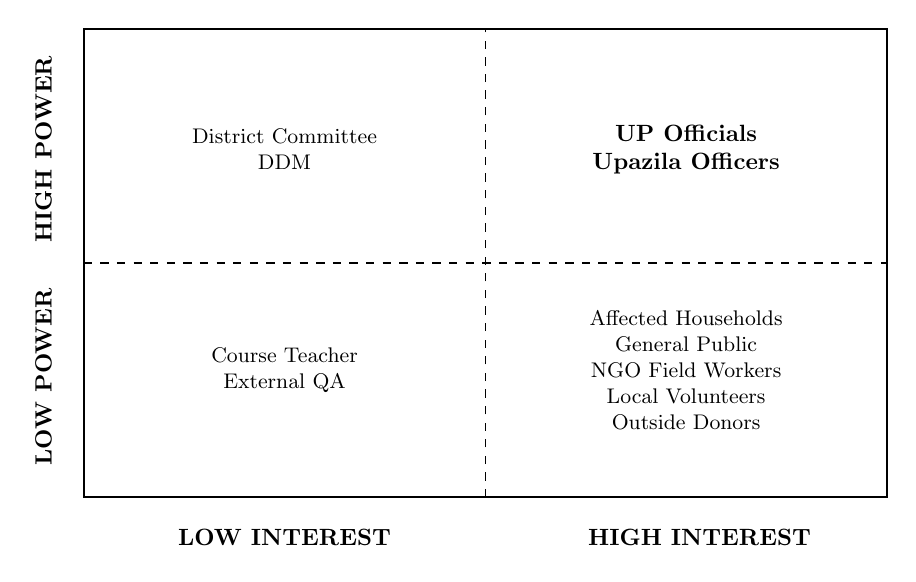
\begin{tikzpicture}[scale=0.85, transform shape]
    \draw[thick] (0,0) rectangle (12,7);
    \node[rotate=90] at (-0.6,5.2) {\textbf{HIGH POWER}};
    \node[rotate=90] at (-0.6,1.8) {\textbf{LOW POWER}};
    \node at (3,-0.6) {\textbf{LOW INTEREST}};
    \node at (9.2,-0.6) {\textbf{HIGH INTEREST}};
    \draw[dashed] (0,3.5) -- (12,3.5);
    \draw[dashed] (6,0) -- (6,7);

    % --- High Power / High Interest (Manage Closely) ---
    \node[align=center, font=\bfseries] at (9,5.2) {UP Officials\\Upazila Officers};

    % --- High Power / Low Interest (Keep Satisfied) ---
    \node[align=center, font=\small] at (3,5.2) {District Committee\\DDM};

    % --- Low Power / High Interest (Keep Informed) ---
    \node[align=center, font=\small] at (9,1.9) {Affected Households\\General Public\\NGO Field Workers\\Local Volunteers\\Outside Donors};

    % --- Low Power / Low Interest (Monitor) ---
    \node[align=center, font=\small] at (3,1.9) {Course Teacher\\External QA};
\end{tikzpicture}
\captionof{figure}{Power-Interest Grid of ReliefMesh Stakeholders}
\label{fig:power-interest}
\end{center}

\section{User Persons}

\subsection{Person 1 --- Rahim Uddin (UP Official)}
\begin{itemize}[nosep]
    \item \textbf{Age:} 42 \textbar{} \textbf{Device:} Android smartphone (basic)
    \item \textbf{Connectivity:} 2G/3G intermittent; no internet during flooding
    \item \textbf{Goal:} Register all affected families quickly and log distributions
    \item \textbf{Key Need:} Offline data entry, simple Bengali-labeled form, photo capture
\end{itemize}

\subsection{Person 2 --- Nasrin Akter (NGO Worker, BRAC)}
\begin{itemize}[nosep]
    \item \textbf{Age:} 28 \textbar{} \textbf{Device:} Android tablet
    \item \textbf{Goal:} Log distributions without duplicating with UP teams
    \item \textbf{Key Need:} Duplicate alert before distribution, cross-agency visibility
\end{itemize}

\subsection{Person 3 --- Kamal Hossain (Upazila Officer)}
\begin{itemize}[nosep]
    \item \textbf{Age:} 51 \textbar{} \textbf{Device:} Desktop PC at office
    \item \textbf{Goal:} Verify that all unions under jurisdiction are distributing correctly
    \item \textbf{Key Need:} Dashboard showing all UP activity, export to PDF
\end{itemize}

\subsection{Person 4 --- Fatema Begum (Journalist / Public)}
\begin{itemize}[nosep]
    \item \textbf{Age:} 34 \textbar{} \textbf{Goal:} Verify relief is reaching affected areas
    \item \textbf{Key Need:} Public dashboard with map and item-level summary by union
\end{itemize}

\subsection{Person 5 --- Arif Hossain (Outside Individual Donor)}
\begin{itemize}[nosep]
    \item \textbf{Age:} 30 \textbar{} \textbf{Goal:} Send relief to home village without duplicating
    \item \textbf{Key Need:} Public heatmap + simple pledge form
\end{itemize}

\section{Stakeholder Requirements Summary}
\begin{table}[H]
\centering
\caption{Stakeholder Requirements Summary}
\label{tab:stakeholder-reqs}
\begin{tabularx}{\textwidth}{@{}lX@{}}
\toprule
Stakeholder & Core Requirements \\
\midrule
UP Official & Offline household registration, photo+GPS distribution log, Bengali UI \\
Upazila Officer & Audit trail, jurisdiction-filtered dashboard, PDF export \\
NGO Worker & Cross-agency duplicate alert, own distribution log \\
General Public & Dashboard (no login), union-level summary, map view \\
District Committee & Aggregated district report, no household PII \\
Outside/Local Volunteers & Heatmap of need, simple pledge form \\
\bottomrule
\end{tabularx}
\end{table}
